%   Filename    : chapter_4.tex 
\chapter{Research Methodology}
This chapter lists and discusses the specific steps and activities that will be performed to accomplish the project. 
The discussion covers the activities from pre-proposal to Final SP Writing.

\section{Research Activities}
\begin{figure}[htbp]
	\centering
	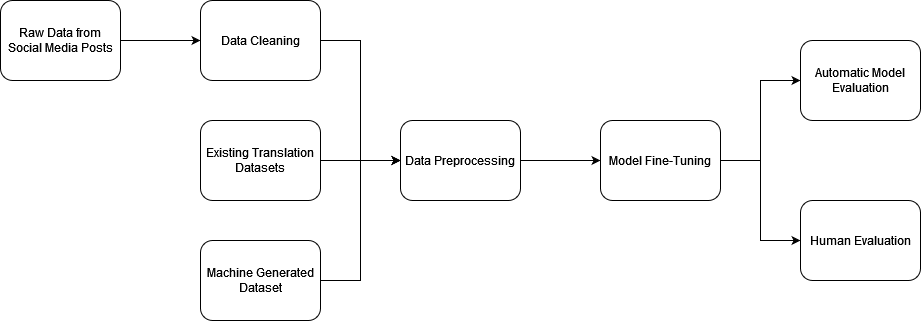
\includegraphics[scale=0.5]{figures/methodology.png}
	\caption{Summarized Methodology}
\end{figure}
\subsection{Data Gathering} 
A dataset of sentences containing Generation Z slang and its formal translation was used in this study. 
This dataset was created using several source: data obtained from social media posts and manually translated by the researchers, existing datasets from HuggingFace, and machine generated and translated sentences using GPT-4o from OpenAI.

The data obtained from social media posts were from verified users of X whose ages are within the Generation Z, so that the dataset is accurate. The data was manually translated by the researchers to ensure that the translation is accurate and reflective of the target demographic. This study also takes into account the regional, cultural, and temporal variations inherent in Gen Z internet slang. The dataset was sourced mostly from individuals whose slang expressions are heavily influenced by contemporary pop culture, including social media trends, music, gaming, and online communities. Temporally, the dataset covers slang used from 2020 through 2024, capturing the evolution of language over recent years and allowing the model to account for shifts in slang popularity and meaning within this period. We, then, used the consensus of the translators and the surrounding environment in which it was created. For social media posts, we considered other comments made by the poster to determine the context in which the word is used in. Its translation is then created using the translator’s own experience. To ensure correctness and accuracy of the translations, each term was cross-referenced with reliable online sources, such as online slang dictionaries, forums, and context-specific usage on social media platforms. This process helped confirm that the translated meanings aligned with commonly accepted interpretations and real-world usage, thus enhancing the validity of the dataset. 

Data obtained from existing datasets and GPT-4o was checked manually to check if whether the sentence is one used by Generation Z. These processes ensured that the dataset is of high quality and representative of what and how Generation Z slang is used.

\subsection{Data Preprocessing} 
The dataset used for the fine-tuning of the model was preprocessed to ensure optimal performance of the model.
Unnecessary information such as email addresses and URLs was removed. The data was then manually cleaned up to remove unnecessary characters such as emojis and fixed issues such as typos. A similar approach was done with existing and machine generated datasets to ensure consistency within the training dataset.

The dataset is then split into train and test datasets in a 90/10 ratio to maximize the data learned by the model without compromising on the model's ability to generalize to new data. The train dataset is then split again into a 90/10 ratio to ensure no overfitting while still allowing the model to adapt to the pattern of slang. The cleaned up dataset was then tokenized through the Transformers library provided by HuggingFace as the library already has tokenizers available for their pretrained models.
This ensures that the data is formatted properly as required by the model to be used.

\subsection{Model Fine-Tuning}
The model used in this study was zephyr-7b-beta because it is open-source and was proven to perform better than other models of the same size. The LLM is capable of understanding how a slang word is used through the surrounding words. This ensures that as long as the word is used within the same context, it will have the correct interpretation. In addition, it can be trained in a GPU with 16GB of VRAM, necessary as we are using the free plan of Google Colab as the platform of choice for prototype fine-tuning of the model. However, during the training process with the full dataset, the Pro+ plan of Google Colab was used for faster training time and background execution of the training process, allowing the training to continue uninterrupted regardless of the network connection.
This study used the example codes provided by HuggingFace in the documentation of their various libraries and sample notebook provided in the zephyr-7b-beta repository. 

The SFTTrainer has EarlyStoppingCallback built in that stops the model training when the evaluation criteria set for the callback stop improving more than the specified threshold for a specified number of epochs regardless of if the training loss is still lowering. After it stops the model training, it will load the model with the best score in terms of the evaluation criteria. This ensures that no overfitting occurs as the validation dataset is independent of the training dataset.

The model was loaded using the Transformers library and was quantized into 4 bits through BitsandBytes library to fit the entire model in the allocated resources while having enough headroom for training. In addition, the Unsloth library was used to speed up the training time and reduce the resources used even more \cite{unsloth}. A LoRA adapter was then attached to the model to further reduce the parameters to be trained.

To evaluate the model training process and ensure that the model is not overfitting, BLEU and ROUGE will be used. These metrics use n-grams, making them superior to standard recall and precision metrics as they take into account the positioning of the words. These two metrics were implemented using the Evaluate library by HuggingFace, making it easier to integrate with the rest of the model training process. These metrics was calculated at every epoch of the training process and is used for an early stopping callback to immediately stop the model training if the model seems to be overfitting.

The model was then trained using SFTTrainer class from the Transformer Reinforcement Learning (TRL) library of HuggingFace to simplify the training process \cite{vonwerra2022trl}. The model was trained with the following parameters: optimizer is paged 4bit AdamW, batch size of 8, learning rate of 2e-5, and maximum number of epochs of 50. These parameters were chosen based on the GPU provided in Colab, the test notebook by HuggingFace and the default parameters of SFTTrainer.

\subsection{Model Evaluation}
The model was evaluated using both automatic and manual evaluation metrics. Identical answers and answers with minimal difference, such as punctuation, between the fine-tuned and the base model were removed in the test set to ensure that the model is evaluated properly. After filtering, a total of 143 sentences were used to evaluate the model. The model was then prompted to generate a formal sentence for 170 sentences in the test dataset. The generated sentences were then compared to the formal translation of the sentence using BLEU and ROUGE metrics. The base zephyr-7b-beta model was also prompted to generate sentences for the BLEU and ROUGE metric and the pairwise comparison for human evaluation. 

An online survey was conducted using Google Forms to compare the outputs of the fine-tuned model and the base model in order to evaluate the effectiveness of the fine-tuning process. Participants were presented with sentence pairs generated by both models and were asked to choose the more accurate translation of a given Generation Z slang sentence based on accuracy, naturalness, and contextual appropriateness. To minimize potential ordering bias, the sequence in which the outputs from the two models were displayed was randomized for each pair. The researchers implemented a Split Questionnaire Design (SQD) by dividing the full survey into multiple sets to improve response rates and reduce respondent fatigue \cite{Peytchev_Peytcheva_2017}. A total of 143 questions was unevenly distributed into six forms. In addition, the number of responses per form varied which leads to an unbalanced results with some items being evaluated more than others.

To address these challenges, aggregated weighted average was utilized. In weighted average, the results of each form was weighted so that responses are represented proportionately \cite{Ganti_2024}. Specifically, the responses to each item were first summarized using their average scores. These scores were then weighted by the number of respondents per item to account for variations in form size and respondent count. This weighting approach allowed us to combine results from the six forms in a way that gave appropriate emphasis to the sample size behind each item’s score, providing a fair and interpretable basis for comparison across all 143 questions.

This method offered a simple yet effective way to integrate responses from an SQD structure without requiring overlap or complex modeling assumptions. It also ensured that items answered by more respondents contributed more substantially to the overall evaluation while avoiding bias from unequal form lengths.
